\documentclass[9pt,twocolumn,twoside]{optica}

\usepackage[english]{babel}
\usepackage{listings}
\usepackage{color}

\setboolean{shortarticle}{false}
\setboolean{minireview}{false}

\title{Laboratorio 1 - Fuerza Bruta}

\author{Juan Retamales}
\affil{Profesora: Mónica Villanueva}
\affil{Ayudante: Patricio Vargas}

\definecolor{mygreen}{rgb}{0,0.6,0}
\definecolor{mygray}{rgb}{0.5,0.5,0.5}
\definecolor{mymauve}{rgb}{0.58,0,0.82}

\definecolor{mybackground}{rgb}{245,245,245}

\lstset{ %
  backgroundcolor=\color{mybackground},   % choose the background color
  basicstyle=\footnotesize,        % size of fonts used for the code
  breaklines=true,                 % automatic line breaking only at whitespace
  captionpos=b,                    % sets the caption-position to bottom
  commentstyle=\color{mygreen},    % comment style
  escapeinside={\%*}{*)},          % if you want to add LaTeX within your code
  keywordstyle=\color{blue},       % keyword style
  stringstyle=\color{mymauve},     % string literal style
}


% To be edited by editor
% \dates{Compiled \today}

% To be edited by editor
% \doi{\url{http://dx.doi.org/10.1364/optica.XX.XXXXXX}}

\begin{abstract}
	\par{En }
      este documento se da a conocer conceptos básicos del algoritmo fuerza bruta y el lenguaje de programación C para combinarlos y realizar una actividad en un entorno  de desarrollo con condicionantes y propiedades. Para así poder analizarlo y llegar a conclusiones sobre su uso y viabilidad.
\end{abstract}

\setboolean{displaycopyright}{true}

\begin{document}

\maketitle

\section{Introducción}{
	\par{En}
    el presente documento veremos cómo se fusiona un algoritmo de combinatoria llamado fuerza bruta con un lenguaje de programación llamado C, y así poder realizar una actividad en un entorno de desarrollo claramente explicado para comprender la importancia y el costo de recursos además de complejidad del algoritmo fuerza bruta.
Usando una combinatoria con condiciones para discriminar resultados lograremos usar una “pseuda-fuerza bruta” para llegar a algunas conclusiones.

}

\section{Descripción del problema}
Se debe resolver el enunciado de la subsección A, antes del plazo de entrega informado en la subsección D.
\subsection{Enunciado}
La empresa
Cuidate SA
crea sistemas de seguridad básicos basados en com-
binaciones de números. Se sabe que el largo de las contraseñas es de 12 unidades
y además se deben cumplir ciertos criterios para formar las claves. En primer
lugar no se pueden generar códigos en donde existan 3 números iguales consecu-
tivos, la segunda condición indica que si la contraseña comienza con un número
impar no puede terminar con un número impar, por último, la combinación no
puede contener secuencias de más de 3 números, por ejemplo, si en la contraseña
se forma la secuencia 1234 significa que la clave es inválida. Considerando que
los números están entre el 0 al 9 diseñe e implemente un programa que encuentre
todas la posibles combinaciones dado un conjunto de entrada, para esto utilice
la técnica de Fuerza Bruta y el lenguaje de programación C \cite{actividad}.

\subsection{Entrada}
En un archivo de texto titulado
entrada.in
se encuentran listados todos
números que se deben utilizar para formar las contraseñas.
\subsection{Salida}
En un archivo de texto titulado
salida.out
se debe mostrar separadas por
saltos de líneas todas las contraseñas que se pueden crear con el archivo de
entrada. Si con el contenido de la entrada no se pueden construir un conjunto
de claves se debe informar en el archivo que se necesita otro conjunto.



%tabla
\begin{table}
\centering
\caption{Ejemplo de entrada y salida }
\label{my-label}
\begin{tabular}{|c|c|lll}
\cline{1-2}
entrada & salida &  &  &  \\ \cline{1-2}
0         &          &  &  &  \\ \cline{1-2}
1         & 125433221002         &  &  &  \\ \cline{1-2}
2         & 431023312115         &  &  &  \\ \cline{1-2}
3         & 652323119011         &  &  &  \\ \cline{1-2}
4         & 514173319930         &  &  &  \\ \cline{1-2}
5         & 001122334455         &  &  &  \\ \cline{1-2}
6         & ...............         &  &  &  \\ \cline{1-2}
\end{tabular}
\end{table}

\subsection{Entrega}
Domingo 9 de abril del 2017 hasta las 23:59, se descontará 1 punto
por cada hora de retraso, al no entregar se reprueba el laboratorio.


\section{Marco Teorico}
Se pretende mediante el enunciado anterior, comprender sobre el funcionamiento del algoritmo de fuerza bruta usando el lenguaje de programación C.

\subsection{Fuerza Bruta}
Es un algoritmo de combinatoria mas simple de diseñar, pero la más costosa ya que equivale a realizar una búsqueda exhaustiva, es decir examinar todas las posibilidades, evaluar cada una de ellas y después escoger alguna que se adapte a los requerimientos. Esto es ineficiente si el número de configuraciones o de posibles soluciones es grande. 
Sin embargo, el proceso de intentar una solución con fuerza bruta también puede resultar adecuado como primera aproximación a la solución final, porque permite profundizar sobre el problema y conocer propiedades útiles para desarrollar un algoritmo más eficiente \cite{algoritmo}.

\subsection{Lenguaje de programación C}
El lenguaje C es un lenguaje estructurado, en el mismo sentido que lo son otros
lenguajes de programación tales como el lenguaje Pascal, el Ada o el Modula-2, pero
no es estructurado por bloques, o sea, no es posible declarar subrutinas (pequeños
trozos de programa) dentro de otras subrutinas, a diferencia de como sucede con otros lenguajes estructurados tales como el Pascal. Además, el lenguaje C no es rígido en la comprobación de tipos de datos, permitiendo fácilmente la conversión entre diferentes tipos de datos y la asignación entre tipos de datos diferentes \cite{lenguajeC}.
\begin{lstlisting}[language=C]
#include <stdio.h>
#include <stdlib.h>
#include <string.h>
#include <ctype.h>
int main(int argc, char** argv) {
    ...
    return (EXIT_SUCCESS); 
}
\end{lstlisting}

\section{Descripción de la solución}
\subsection{Etorno}

El entorno de trabajo se realizó en el editor Netbeans IDE 8.2 en su versión de 64 bits en el cual se le instalo el software Cygwin el cual proporciono un compilador del lenguaje C y herramientas necesarias por Netbeans para el trabajo.
Todo lo anterior mencionado se montó en un computador AMD de 4 núcleos de 2.9 Ghz con 16Gb de memoria ram el cual tiene instalado el sistema operativo Windows 7 en su versión Ultimate de 64bits y más de 500Gb de espacio libre en el disco duro principal.

Netbeans al ser un entorno de desarrollo de alto nivel, crea automáticamente muchos archivos que no son necesarios para esta “simple” actividad, por lo que solo destacaremos 3 de ellos:

-\textbf{main.c}: Guarda el código del algoritmo así como todas las funciones utilizadas.

-\textbf{entrada.in}: Se utilizara para leer los números para leer la combinatoria, cabe destacar que para no incidir a un error se utilizara el archivo en formato UTF sin BOM.
En este archivo de texto se leen todos los caracteres, de los cuales se extraen todos los números entre 0 y 9, de ser un numero de dos dígitos quedaran como dos de un digito, y de los dígitos guardados no se podrán repetir, es decir si ingreso 33 solo se guardara una vez 3.

-\textbf{salida.out}: Es el archivo que guardara todas las combinaciones validas con un salto de linea entre cada combinación.

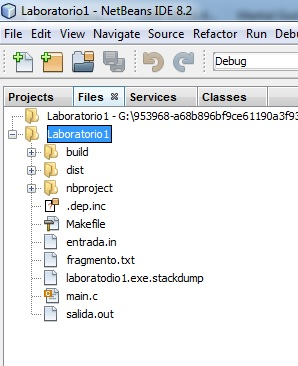
\includegraphics[scale=1.1]{archivos.jpg}

\subsection{Condiciones}
Del enunciado se pueden extraer tres condiciones que se debe cumplir para que la combinatoria sea válida:
\begin{enumerate}
\item No se pueden generar códigos en donde existan 3 números iguales consecutivos.
\item Si la contraseña comienza con un número impar no puede terminar con un número impar.
\item La combinación no puede contener secuencias de más de 3 número.
\end{enumerate}
Para cada una de estas condiciones se utilizó una función llamada “validadorIgualesConsecutivos”, “validadorImparImpar” y “validadorConsecutivos” respectivamente, que retornaban 0 de ser válido y 1 de no serlo.

\begin{lstlisting}[language=C]
/*
 * validadorImparImpar - verifica que si el primer numero es impar, no termine en impar
 *
 *Entrada: 2 numeros de formato int.
 *Saluda: Numero int 0 o 1.
 */
int validadorImparImpar(int c1, int c12)
{
    if(c1%2==1 && c12%2==1)
    {
        return 1;
    }
    return 0;
}
\end{lstlisting}

Una cuarta validación podría ser que tenga 12caracteres de longitud o que sea conformado por números desde el 0 al 9 inclusive, pero por la construcción del software, siempre crea combinaciones de 12 digitos y el archivo entrada.in lo lee carácter por carácter haciendo que si intenta entrar un numero de dos dígitos, contara como dos números y no como un numero de dos dígitos.

\subsection{Logica}
Para generar las combinaciones se utilizaron 12 ciclos anidados que comprendía el largo de caracteres que podía utilizar la combinación, es decir, si la combinación el largo fuera 7, solo hubieran sido necesarios 7 ciclos anidados. Cada ciclo “for” utilizo una variable del abecedario para identificarla y utilizarla, la cual consto de la letra “a” a la letra “l”.

Además al realizar la combinación, se revisó si dicho numero era válido y de serlo, se guardaba en el archivo salida.out. Cada combinación está separada por un salto de línea para realizar la lectura al ojo humano mas ligera.

\begin{lstlisting}[language=C]
fp = fopen ( "salida.out", "a" );
sprintf(str, "%d", entrada[a]);
fprintf(fp, "%s", str);
sprintf(str, "%d", entrada[b]);
fprintf(fp, "%s", str);
sprintf(str, "%d", entrada[c]);
fprintf(fp, "%s", str);
sprintf(str, "%d", entrada[d]);
fprintf(fp, "%s", str);
sprintf(str, "%d", entrada[e]);
fprintf(fp, "%s", str);
sprintf(str, "%d", entrada[f]);
fprintf(fp, "%s", str);
sprintf(str, "%d", entrada[g]);
fprintf(fp, "%s", str);
sprintf(str, "%d", entrada[h]);
fprintf(fp, "%s", str);
sprintf(str, "%d", entrada[i]);
fprintf(fp, "%s", str);
sprintf(str, "%d", entrada[j]);
fprintf(fp, "%s", str);
sprintf(str, "%d", entrada[k]);
fprintf(fp, "%s", str);
sprintf(str, "%d", entrada[l]);
fprintf(fp, "%s", str);
fprintf(fp, "\n");
fclose ( fp );
\end{lstlisting}

Y aunque no es realmente fuerza bruta por que el computador no lo permite desde el procesador al disco duro, ya que tendríamos que guardar todas las combinaciones no solo con los números ingresados, si no con todas las combinaciones de 0 a 9 posibles además de posteriormente verificarlas. 

Al menos pasamos por todas las combinaciones posibles con los números entrantes y aunque se acoto en gran medida el proceso, sigue siendo una enorme carga para el equipo. 

\section{Análisis de los resultados}

En la \textbf{Table 2.} Ejemplos de salida, se muestran 6 de los resultados aleatorios obtenidos con los números de entrada 1,3 y 8. 

%tabla
\begin{table}
\centering
\caption{Ejemplos de salida }
\label{my-label}
\begin{tabular}{|c|c|lll}
\cline{1-2}
N° & Resultado &  &  &  \\ \cline{1-2}
1         & 113113113118         &  &  &  \\ \cline{1-2}
51         & 113113188138         &  &  &  \\ \cline{1-2}
86         & 113113383318         &  &  &  \\ \cline{1-2}
147         & 113113883388         &  &  &  \\ \cline{1-2}
184         & 113118138838         &  &  &  \\ \cline{1-2}
122454         & 883883883883         &  &  &  \\ \cline{1-2}
\end{tabular}
\end{table}

Y visualmente todos cumplen con las condiciones impuestas anteriormente para ser una combinación valida.

\section{Traza de la solución}

Primero revisa un archivo de texto llamado entrada.in del cual se leen todos los caracteres, como de los cuales se extraen todos los números entre 0 y 9, y se guardan en un arreglo, además de un contador para saber el largo de este arreglo.
Luego crea o sobrescribe el archivo salida.out para guardar las combinaciones, borrando cualquier registro anterior que tuviera.


Luego pasa por los 12 ciclos “for” anidados con variables de la “a” a “l”, donde al igual que se resuelve un candado de combinación, se cada vez que un ciclo se termina, el anterior avanza una vez y llama al arreglo de combinación por cada digito para así formar cada combinatoria. Por ejemplo si de entrada tenemos el número 1 y 2, la primera combinación seria “111111111111” y la segunda “111111111112”, la tercera “111111111121” y así sucesivamente.


Luego de formar cada combinación realiza tres validaciones de las condiciones que se mencionaron anteriormente, y si las logra cumplir, escribe la combinación en el archivo salida.out y posteriormente realiza un salto de línea para diferenciarlos entre cada combinación. En este caso una combinación que cumpliera las condiciones se escribiría “112211221122” y despues un salto de linea.

\begin{lstlisting}[language=C]
fp = fopen ( "salida.out", "a" );
/*entrada[a] seria 1*/
sprintf(str, "%d", entrada[a]);
fprintf(fp, "%s", str);
/*entrada[b] seria 1*/
sprintf(str, "%d", entrada[b]);
fprintf(fp, "%s", str);
/*entrada[c] seria 2*/
sprintf(str, "%d", entrada[c]);
fprintf(fp, "%s", str);
/*entrada[d] seria 2*/
sprintf(str, "%d", entrada[d]);
fprintf(fp, "%s", str);
/*entrada[e] seria 1*/
sprintf(str, "%d", entrada[e]);
fprintf(fp, "%s", str);
/*entrada[f] seria 1*/
sprintf(str, "%d", entrada[f]);
fprintf(fp, "%s", str);
/*entrada[g] seria 2*/
sprintf(str, "%d", entrada[g]);
fprintf(fp, "%s", str);
/*entrada[h] seria 2*/
sprintf(str, "%d", entrada[h]);
fprintf(fp, "%s", str);
/*entrada[i] seria 1*/
sprintf(str, "%d", entrada[i]);
fprintf(fp, "%s", str);
/*entrada[j] seria 1*/
sprintf(str, "%d", entrada[j]);
fprintf(fp, "%s", str);
/*entrada[k] seria 2*/
sprintf(str, "%d", entrada[k]);
fprintf(fp, "%s", str);
/*entrada[l] seria 2*/
sprintf(str, "%d", entrada[l]);
fprintf(fp, "%s", str);
/*y realiza el salto de linea.*/
fprintf(fp, "\n");
fclose ( fp );
\end{lstlisting}

\section{Conclución}

La fuerza bruta es un método de combinación que realiza todas las posibilidades de combinatoria de un elemento, a pesar de ser simple, requiere un gran gasto tiempo y recursos del equipo, y aun que el codigo podria ser optimizado para otras situaciones, se puede concluir que realizar las combinaciones de 12 dígitos de longitud aun cuando acotamos el proceso de tal manera que en verdad usamos una “pseuda-fuerza bruta” requirió un enorme gasto de procesamiento por lo que sin lugar a dudas nos lleva a buscar un algoritmo más eficiente o al menos, a tratar de no usarlo a menos de ser necesario.
La actividad demostró sin lugar a dudas lo anterior mencionado y de no ser por las validaciones y acotar la fuerza bruta, podría haber sido imposible realizar dicho proceso en computadores cotidianos o al menos en el equipo usado.



% Bibliography
\bibliography{sample}

% Full bibliography will be added automatically for Optics Letters submissions
% Note that this extra page will not count against page length
\bibliographyfullrefs{sample}

\end{document}